% !TeX program = xelatex
\documentclass[12pt,a4paper]{ctexart}
\usepackage[top=2.4cm,bottom=2.4cm,left=2.4cm,right=2.4cm]{geometry}
\usepackage{graphicx}
\usepackage{amsmath,amssymb}
\usepackage{booktabs}
\usepackage{longtable}
\usepackage{array}
\usepackage{float}
\usepackage{caption}
\usepackage{enumitem}
\usepackage{xcolor}
\usepackage[colorlinks=true,linkcolor=black,citecolor=black,urlcolor=black]{hyperref}
\graphicspath{{../figures/}}

\captionsetup{font=small,labelsep=quad}
\setlength{\parskip}{0.25em}
\renewcommand{\thefigure}{\arabic{figure}}
\ctexset{section={format=\Large\bfseries\heiti,name={,、},number=\chinese{section}}}

\newcommand{\wj}[1]{\textbf{#1}}
\newcommand{\dd}{\mathrm{d}}

\begin{document}

\begin{center}
{\zihao{2}\heiti 2026 年新手数学建模竞赛 \quad A 题}\\[0.5em]
{\zihao{3}\heiti 乳酸发酵工艺的规律与优化}\\[0.6em]
{\zihao{5} ——基于生长—产酸—耗糖耦合动力学与多目标工艺优化的建模全过程}
\end{center}

\vspace{0.3em}

% ==========================================================
\begin{center}\zihao{4}\heiti 摘\quad 要\end{center}

本文针对乳酸分批发酵的“菌体生长—产酸—耗糖”规律与工艺决策问题，按“单变量规律 $\to$ 耦合机理 $\to$ 参数优化 $\to$ 过程强化”的递进逻辑建立了一组相互衔接的数学模型，并对全部参数给出了最小二乘估计、置信区间与模型检验。

\wj{针对问题 1}，将菌体浓度取对数后视为一维状态量，比较了指数模型、含迟滞期指数模型、Logistic 模型、Gompertz 模型与 Richards 模型五类生长模型。以残差平方和最小为准则、以 AIC 为选择准则，Logistic 模型取胜：
$L(t)=L_0+A/[1+e^{-k(t-t_m)}]$，
参数估计为 $L_0=7.582,\ A=2.106,\ k=0.683\ \mathrm{h^{-1}},\ t_m=5.511\ \mathrm{h}$，
$R^2=0.99982$、$\mathrm{RMSE}=0.011\ \lg(\mathrm{CFU/mL})$、留一交叉验证 RMSE 仅 $0.027$，残差无系统性趋势。
由模型求得最大比生长速率 $\mu_m=0.360\ \lg(\mathrm{CFU/mL})\cdot\mathrm{h^{-1}}$（在 $t=5.51$ h 处取得，相当于 $\mu=0.828\ \mathrm{h^{-1}}$、倍增时间 $0.84$ h），最终菌体量 $L_\infty=9.688$，即 $4.87\times10^{9}$ CFU/mL，较接种时增长约 114 倍。

\wj{针对问题 2}，先由数据识别出“产酸—耗糖”近乎严格成比例的关系，得乳酸得率 $Y_{P/S}=0.989\ \mathrm{g/g}$（$R^2=0.9988$），与同型乳酸发酵的理论值 $1.0\ \mathrm{g/g}$ 吻合。进一步建立带产物抑制的 Luedeking--Piret 耦合模型
$$\frac{\dd P}{\dd t}=\left(\alpha\frac{\dd L}{\dd t}+\beta X\right)\left(1-\frac{P}{P_m}\right),\quad
\frac{\dd S}{\dd t}=-\frac{1}{Y_{P/S}}\frac{\dd P}{\dd t}-m_s,\quad X=10^{L-L_0},$$
以问题 1 的 $L(t)$ 为输入，用变步长 Runge--Kutta 法积分并联合最小二乘估计得
$\alpha=2.269$、$\beta=0.0466\ \mathrm{h^{-1}}$、$P_m=9.912\ \mathrm{g/L}$、$Y_{P/S}=1.056$、$m_s=0.0459\ \mathrm{g/(L\cdot h)}$。
模型对乳酸与残糖的 $R^2$ 分别为 $0.9955$ 与 $0.9946$，逐点相对误差绝对值不超过 $11\%$。
产物抑制阈值 $P_m\approx9.9\ \mathrm{g/L}$ 定量解释了本批发酵“只用了 10.1 g/L 糖、还剩 24.9 g/L 糖就停下来”的现象；产酸来源中生长偶联项占 $31.8\%$、非生长偶联项占 $68.2\%$。

\wj{针对问题 3}，用试验二六个初糖水平的终点数据，依次建立终点产量、终点时间与平均速率模型。终点产量满足“产率—上限”分段规律
$P_\infty=\min\{Y S_0,\ P_{cap}\}$，$Y=0.961$、$P_{cap}=109.9\ \mathrm{g/L}$（$R^2=0.9997$），临界初糖 $S_0^*=P_{cap}/Y=114.3$ g/L，据此预测 150 g/L 时残糖 $35.7$ g/L，与实测 $35.7$ g/L 完全一致。
将终点时间视为“产酸速率降到规定阈值”的时刻，建立含底物抑制与产物抑制的动力学模型（$V_{max}=3.66$、$K_s=2.28$、$K_i=514$、$P_{cap}=111.5$、$Y=0.983$），对终点时间、终点产量、最大速率的 $R^2$ 分别为 $0.954$、$0.998$、$0.546$。
高糖残糖剩余的原因被归结为“产物抑制造成的效价天花板”而非“糖用不完”：当 $S_0>114$ g/L 时，多余的糖在酸达到上限后无法继续转化。
在此基础上以“单位时间净收益”与“单位产品成本”为目标，在 $(S_0,t)$ 平面上做二维寻优，得到经济最优初糖约 $74$--$89$ g/L、放罐时间 $36$--$60$ h，并给出成本参数敏感性：最优初糖在 $58$--$109$ g/L 之间随下游成本与产品价格移动。

\wj{针对问题 4}，选择“及时移出部分乳酸”的强化策略。用问题 2 的模型模拟把罐内乳酸维持在 $2\sim9$ g/L 的原位分离过程：将乳酸控制在 $4$ g/L 时，单批产酸由 $9.72$ g/L 提高到 $35.6$ g/L（$3.7$ 倍），平均产出强度由 $0.694$ 提高到 $2.07\ \mathrm{g/(L\cdot h)}$（$3.0$ 倍），残余糖由 $25.1$ g/L 降到 $0.5$ g/L。作为对照，补料分批可把 150 g/L 总糖的浪费消除，容积产率由 0.93 提高到 $1.34\ \mathrm{g/(L\cdot h)}$，但受效价天花板限制，增益小于移酸。文中最后讨论了模型的适用范围与局限。

\vspace{0.6em}
\noindent\wj{关键词：}Logistic 生长模型；Luedeking--Piret 方程；产物抑制；Michaelis--Menten 动力学；非线性最小二乘；多目标优化

\newpage
\tableofcontents
\newpage

% ==========================================================
\section{问题重述}

\subsection{问题背景}
某生物制造企业的中试车间采用分批发酵生产食品级乳酸：一次性投入以葡萄糖为主要碳源的培养基，接入乳酸菌后不再补料也不放料，菌体一边生长、一边消耗葡萄糖并产出乳酸，罐内温度恒定，到适当时间整批放出（放罐）。企业积累了两组试验数据：

\begin{itemize}[leftmargin=2em,itemsep=0.1em]
\item \wj{试验一}：标准配方（初糖 35 g/L、37 ℃、菌株 L-1、不控 pH）下的一罐完整发酵，$0\sim14$ h 每 2 h 取样，共 8 个时间点，测定菌体浓度 $\lg(\mathrm{CFU/mL})$、乳酸浓度、累计葡萄糖消耗量与残糖浓度。
\item \wj{试验二}：更早前用另一菌株 L-2（40 ℃、pH 恒定为 9.0 自动流加碱液）在 6 个初糖水平（20、40、60、80、100、150 g/L）下的对比试验，每批只记录终点时间、终点菌体（OD600）、终点乳酸、终点残糖、平均与最大产酸速率。
\end{itemize}

两组试验的菌株、温度与 pH 控制方式均不同，因此数据的适用范围需要分别界定。

\subsection{需要解决的问题}
\begin{enumerate}[leftmargin=2.2em,itemsep=0.15em]
\item \wj{问题 1}：针对试验一建立菌体浓度随时间的模型，估计参数、评价吻合程度，并给出最大生长速率与最终菌体量。
\item \wj{问题 2}：在问题 1 基础上建立乳酸生成与葡萄糖消耗的模型，刻画“生长—产酸—耗糖”的联动，估计参数（如每消耗 1 g 葡萄糖生成的乳酸量），分析各时间点的拟合效果与可靠性。
\item \wj{问题 3}：利用试验二分析初糖浓度对终点产量、平均产酸速率、发酵时长、终点残糖的影响，建立模型刻画“终点产量随初糖升高而增加、平均产酸速率却总体下降”的规律，解释 150 g/L 时残糖明显剩余的原因，并在产量、生产强度与设备周转之间给出推荐的初糖浓度与放罐时间。
\item \wj{问题 4}：选择“中途补加糖料”或“及时移出部分乳酸”之一，说明思路并用模型估计效果，同时讨论模型的局限与适用范围。
\end{enumerate}

% ==========================================================
\section{问题分析}

\subsection{总体思路}
四个问题不是彼此独立的四道题，而是一条从“描述”到“机理”再到“决策”的链条（图 \ref{fig:flow}）：

\begin{enumerate}[leftmargin=2.2em,itemsep=0.12em]
\item \wj{问题 1 解决“状态变量怎么走”}：菌体浓度是全部过程的驱动量，先把 $L(t)$ 刻画准，后面才有输入；
\item \wj{问题 2 解决“三个变量怎么联动”}：以 $L(t)$ 为输入，用 Luedeking--Piret 方程把产酸拆成“与生长偶联”和“与菌体量偶联”两部分，再用化学计量系数把产酸与耗糖锁在一起，并用产物抑制解释速率为何在中后期衰减；
\item \wj{问题 3 解决“参数怎么选”}：把问题 2 的机理结构（底物限制 + 产物抑制）平移到试验二的终点数据上，得到终点产量与发酵时长的解析/半解析规律，再做经济寻优；
\item \wj{问题 4 解决“结构怎么改”}：既然瓶颈是产物抑制，就针对性地移除产物，并用模型量化收益。
\end{enumerate}

\begin{figure}[H]
\centering
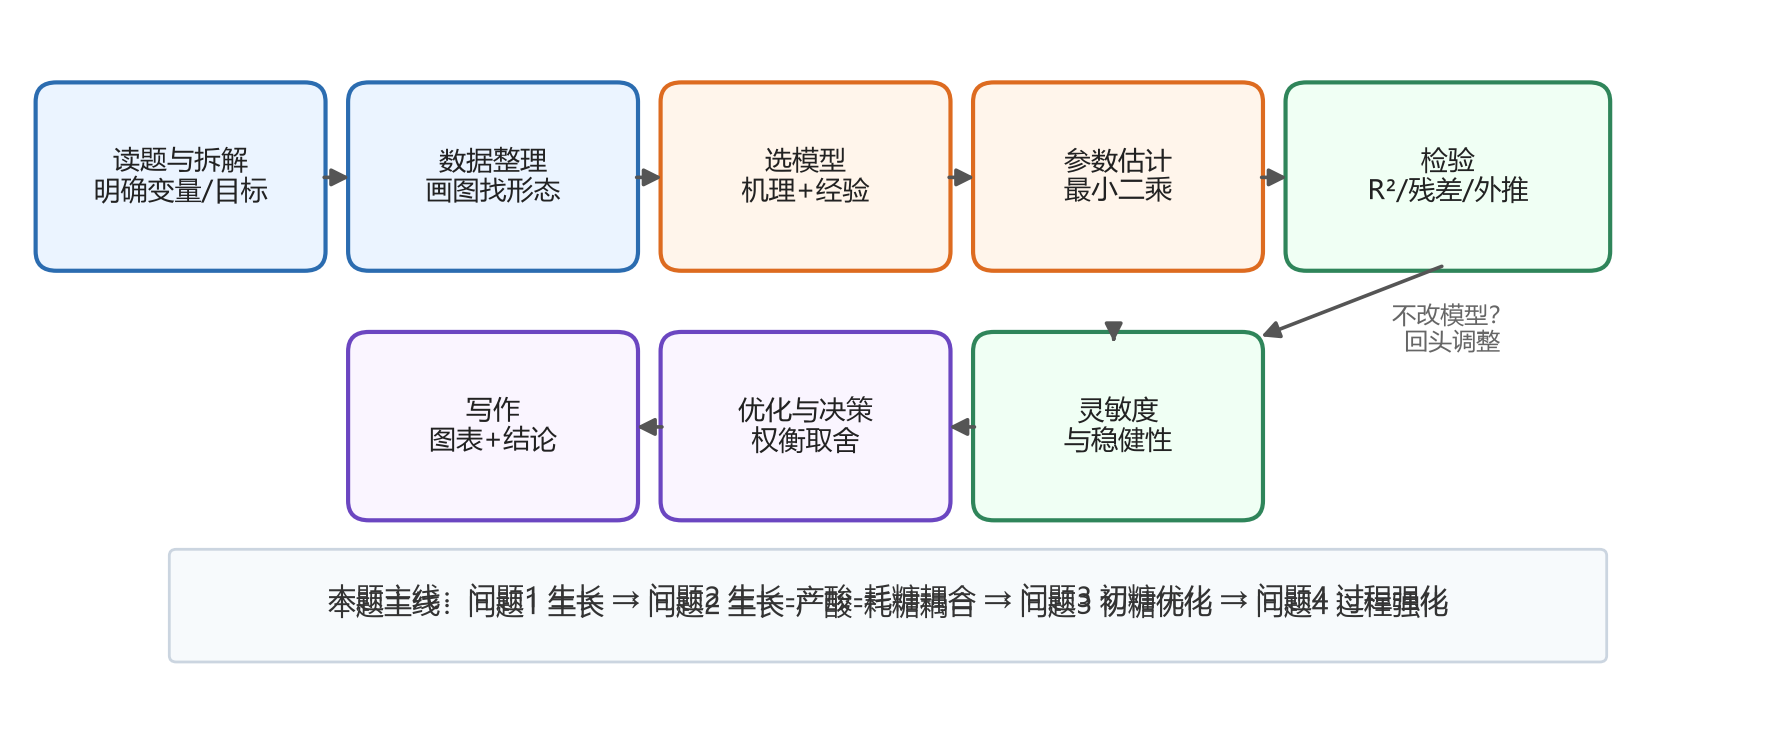
\includegraphics[width=0.97\textwidth]{fig7_workflow.png}
\caption{建模主线与工作流程}
\label{fig:flow}
\end{figure}

\subsection{关键判断}
在动手算之前，先看图 \ref{fig:data} 得到三个定性判断，它们决定了后面的模型形式：

\begin{enumerate}[leftmargin=2.2em,itemsep=0.12em]
\item 菌体曲线是典型的 S 形（迟滞—对数—稳定），既不是纯指数（后期明显变平），也不是纯线性，故应使用饱和型生长模型；
\item 产酸曲线与耗糖曲线形状几乎重合，$P$ 与 $S_c$ 的相关系数达 $0.9996$，提示二者之间存在近似固定的化学计量关系，这将是问题 2 的“锚点”；
\item 试验一在 14 h 时残糖仍有 24.9 g/L 却几乎停止产酸，说明限制因素不是糖；试验二中 150 g/L 时残糖 35.7 g/L 而 100 g/L 时残糖为 0，说明存在一个“酸浓度上限”，而不是“糖越多越好”。
\end{enumerate}

\begin{figure}[H]
\centering
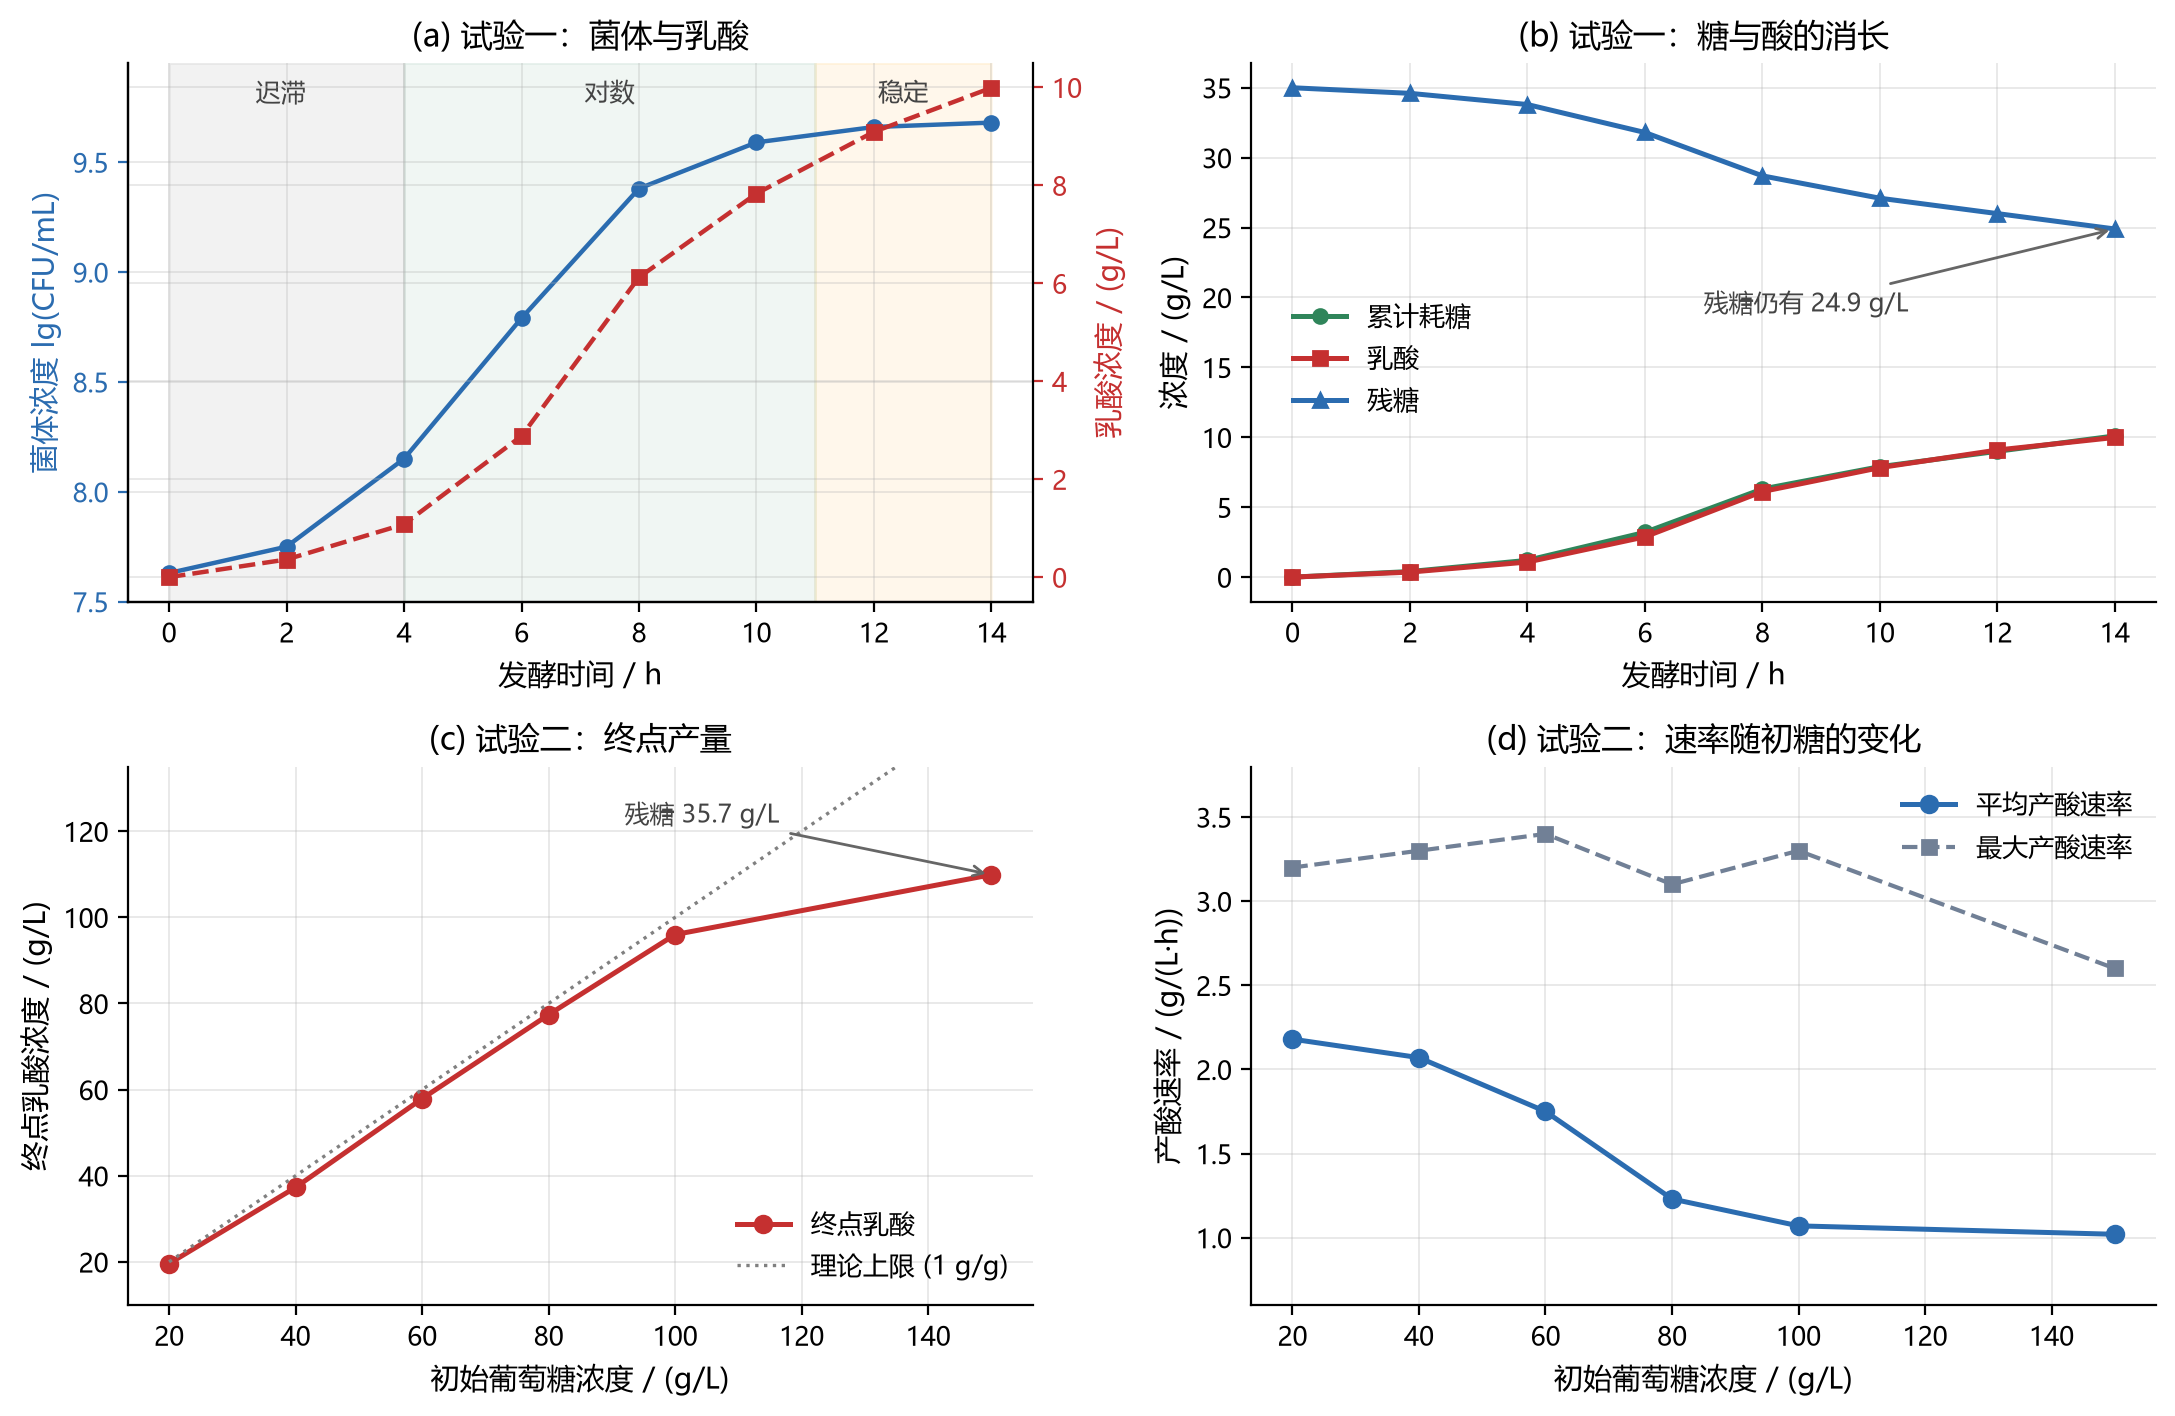
\includegraphics[width=0.98\textwidth]{fig1_data.png}
\caption{两组试验数据的探索性分析。(a)(b) 试验一的时间过程；(c)(d) 试验二的终点指标随初糖浓度的变化}
\label{fig:data}
\end{figure}

% ==========================================================
\section{模型假设}

\begin{enumerate}[leftmargin=2.2em,itemsep=0.15em]
\item \wj{理想混合假设}：发酵罐内搅拌充分，菌体、糖、酸在空间上均匀，可用集总参数（常微分方程）描述，忽略传质与空间梯度。
\item \wj{恒温恒容假设}：温度恒定，分批过程中不补料不放料，体积不变，故浓度即总量除以恒定体积。
\item \wj{单一限制性底物假设}：除葡萄糖外的氮源、无机盐均充足，菌体生长与产酸只受葡萄糖浓度与产物（乳酸）浓度调控。
\item \wj{对数浓度可加性假设}：活菌计数服从对数正态误差，故在对数尺度 $\lg(\mathrm{CFU/mL})$ 上建立模型与做最小二乘，等价于对菌体量取几何平均意义下的最优拟合。
\item \wj{产物抑制的形式假设}：乳酸对生长与产酸的抑制可用线性（或双曲）衰减因子 $1-P/P_m$ 刻画，$P_m$ 为效价上限。
\item \wj{测量误差独立同分布假设}：同一指标的测量误差相互独立、均值为零，菌体约 $\pm0.05\ \lg$ 单位，浓度指标约 $\pm0.15$ g/L，用于加权最小二乘与置信区间估计。
\item \wj{数据可分假设}：试验一与试验二来自不同菌株与不同 pH 策略，二者不混合建模，只做机理上的类比与参数上的迁移说明。
\end{enumerate}

% ==========================================================
\section{符号说明}

\begin{table}[H]
\centering
\caption{主要符号}
\small
\begin{tabular}{l p{9.2cm} p{3.6cm}}
\toprule
符号 & 含义 & 单位 \\
\midrule
$t$ & 发酵时间 & h \\
$L$ & 菌体浓度（以活菌数常用对数计） & $\lg(\mathrm{CFU/mL})$ \\
$X$ & 相对菌体量 $X=10^{L-L_0}$（接种时刻为 1） & -- \\
$S$ & 残糖（葡萄糖）浓度 & g/L \\
$S_c$ & 累计葡萄糖消耗量，$S_c=S_0-S$ & g/L \\
$P$ & 乳酸浓度 & g/L \\
$L_0,A,k,t_m$ & Logistic 模型的下渐近线、增幅、速率常数、拐点时刻 & $\lg$，$\lg$，$\mathrm{h^{-1}}$，h \\
$\mu_m$ & 最大比生长速率（对数尺度） & $\lg\cdot\mathrm{h^{-1}}$ \\
$\alpha,\beta$ & Luedeking--Piret 的生长偶联系数、非生长偶联系数 & $\mathrm{g/L}$\,per\,$\lg$；$\mathrm{h^{-1}}$ \\
$P_m$ & 产物抑制阈值（效价上限） & g/L \\
$Y_{P/S}$ & 乳酸对葡萄糖的得率 & g/g \\
$m_s$ & 维持代谢耗糖速率 & $\mathrm{g/(L\cdot h)}$ \\
$V_{max},K_s,K_i$ & 最大比产酸速率、半饱和常数、底物抑制常数 & $\mathrm{g/(L\cdot h)}$, g/L, g/L \\
$v_{stop}$ & 判定发酵终点的速率阈值 & $\mathrm{g/(L\cdot h)}$ \\
$t_e$ & 发酵终点时间 & h \\
\bottomrule
\end{tabular}
\end{table}

\noindent 说明：$\lg$ 表示以 10 为底的常用对数；为书写方便，正文中 $R^2$ 均指决定系数 $1-\sum(y_i-\hat y_i)^2/\sum(y_i-\bar y)^2$。

% ==========================================================
\section{数据预处理与探索性分析}

\subsection{数据一致性检查}
试验一的残糖由“初糖 35 g/L 减累计消耗量”换算得到，与直接测定值存在定义上的耦合，因此本文只把 $S_c$（累计消耗）视为独立观测，$S$ 作为派生量同时报告。
试验二的 $\mathrm{OD}_{600}$ 与 $\lg(\mathrm{CFU/mL})$ 是两种不可直接比较的计量，本文只在同一试验内部使用，不做跨试验换算。

\subsection{派生指标}
对每一个初糖水平计算毛得率 $Y_{gross}=P/S_0$、净得率 $Y_{net}=P/(S_0-S_r)$、平均产酸速率 $\bar r=P/t_e$。结果见表 \ref{tab:q3data}。

\begin{table}[H]
\centering
\caption{试验二各初糖水平的派生指标}
\label{tab:q3data}
\small
\begin{tabular}{cccccccc}
\toprule
$S_0$/(g/L) & $t_e$/h & OD$_{600}$ & $P$/(g/L) & $S_r$/(g/L) & $P/S_0$ & $\bar r$/(g/(L$\cdot$h)) & OD$/S_c$ \\
\midrule
20  & 9   & 1.99 & 19.6 & 0.1  & 0.980 & 2.178 & 0.100 \\
40  & 18  & 4.19 & 37.3 & 0.0  & 0.932 & 2.072 & 0.105 \\
60  & 33  & 6.25 & 57.9 & 0.0  & 0.965 & 1.755 & 0.104 \\
80  & 63  & 7.69 & 77.4 & 0.5  & 0.968 & 1.229 & 0.097 \\
100 & 90  & 9.19 & 96.0 & 0.0  & 0.960 & 1.067 & 0.092 \\
150 & 108 & 9.72 & 109.9 & 35.7 & 0.733 & 1.018 & 0.085 \\
\bottomrule
\end{tabular}
\end{table}

由表 \ref{tab:q3data} 可得三条经验事实，它们是问题 3 建模的直接依据：
（1）除 150 g/L 外，净得率稳定在 $0.93\sim0.99$，说明糖到酸的转化基本彻底；
（2）终点时间随初糖超线性增长（每翻一番糖，时间增加 2 倍以上）；
（3）单位耗糖的菌体增量（OD$/S_c$）在 $S_0\le100$ 时稳定在 $0.09\sim0.11$，在 150 g/L 时降至 $0.085$，提示高糖存在渗透胁迫。

\subsection{相关性}
相关系数：$r(S_0,P)=0.969$、$r(S_0,\bar r)=-0.916$、$r(S_0,t_e)=0.972$、$r(S_0,r_{max})=-0.741$。
即“产量随初糖升、平均速率随初糖降”是数据的稳健特征，不是个别点的偶然；而最大速率几乎与初糖无关（$3.2\sim3.4$，仅 150 g/L 降为 2.6），说明高糖抑制的是“持续能力”而不是“瞬时能力”，这一点对问题 4 的策略选择很关键。
